\documentclass[a4paper, notitlepage, 11pt]{article}
\usepackage{geometry}
\fontfamily{times}
\geometry{verbose,tmargin=30mm,bmargin=25mm,lmargin=25mm,rmargin=25mm}
\pagestyle{empty}
% end configs
\usepackage{setspace,relsize}               
\usepackage{moreverb}                        
\usepackage{url}
\usepackage{hyperref}
\hypersetup{colorlinks=true,citecolor=blue}
\usepackage{subfigure}
\usepackage{amsmath}
\usepackage{mathtools} 
\usepackage{amsthm}
\usepackage{amssymb}
\usepackage{indentfirst}
\usepackage{todonotes}
\usepackage[authoryear,round]{natbib}
\bibliographystyle{apalike}
\usepackage[pdftex]{lscape}
\usepackage[utf8]{inputenc}

% Title Page
\title{\vspace{-9ex}\centering \bf On the propriety of power priors}
\author{
% Luiz Max de Carvalho\\
% Program for Scientific Computing (PROCC), Oswaldo Cruz Foundation. \\
}
\DeclareMathOperator*{\argmin}{arg\,min}
\DeclareMathOperator*{\argmax}{arg\,max}
\newtheorem{theorem}{Theorem}[]
\newtheorem{proposition}{Proposition}[]
\newtheorem{remark}{Remark}[]
\setcounter{theorem}{0} % assign desired value to theorem counter
\begin{document}
\maketitle

% \begin{abstract}
% 
% Key-words: ;; ; ; . 
% \end{abstract}

\section*{Background}

Power priors are cool. [bunch of citations for propriety of GLM, Cox model, exponential family, etc]

\section*{Results}

The data $D_0 \in \mathcal{X} \subseteq \mathbb{R}^p$  and the parameter $\theta \in \Theta \subseteq \mathbb{R}^q$ and $a_0 \geq 0$.
\begin{equation}
\label{eq:power_prior}
 p(\theta \mid D_0, a_0) \propto L(D_0 \mid \theta)^{a_0}\pi(\theta)
\end{equation}

We want to show under which conditions
\[\int_{\Theta} L( D_0 \mid \theta)^{a_0}\pi(\theta) d\theta <\infty.\]
\begin{theorem}
\label{thm:integrability}
 Assume $\int_{\mathcal{X}} L( x \mid \theta)dx < \infty$.
 Denote $f_{a_0}(D_0;\theta) : = L( D_0 \mid \theta)^{a_0}\pi(\theta)$.
 Then for $a_0 > 0$, $\int_{\Theta} f_{a_0}(D_0;\theta) d\theta <\infty$.
\end{theorem}
\begin{proof}
First, note that for $0 < a_0 \leq 1$, the function $g(x) = x^{a_0}$ is concave.
Then, by Jensen's inequality and the finiteness of $L( D_0 \mid \theta)$ for all of its arguments we have
\[ \int_{\Theta} f_{a_0}(D_0; \theta) d\theta \leq \left[ \int_{\Theta} L(D_0 \mid\theta)\pi(\theta)d\theta \right]^{a_0} < \infty. \]
Rewrite $f_{a_0}(D_0; \theta) = L(D_0\mid\theta)^{a_0 -1} L(D_0\mid\theta)\pi(\theta)$.
If $1 \leq a_0 \leq 2$, we have the Jensen's inequality case above, since we know that $L(D_0\mid\theta)\pi(\theta)$ is normalisable.
Similarly, if $2 \leq a_0 \leq 3$, we can write 
\[  f_{a_0}(D_0; \theta) = L(D_0\mid\theta)^{a_0-p} L(D_0\mid\theta)^p\pi(\theta), \]
with $1 \leq p \leq 2$, again falling into the same case, since we know that $L(D_0\mid\theta)^{p}\pi(\theta)$ is normalisable.
We can then show that for any $n \geq 1 \in \mathbb{N}$, $\int_{\Theta}f_{a_0}( D_0 ; \theta)d\theta < \infty$ for  $n-1 \leq a_0 \leq n$.
The base case for $1 \leq n \leq 3$ is established.
Now suppose the hypothesis holds for $n \geq 3$.
For $n + 1$ we have for $ n \leq  a_0 \leq n + 1$ and $n-1 \leq p_n \leq n$:
\begin{align*}
 \int_{\Theta} L(D_0\mid\theta)^{a_0-p_n} L(D_0\mid\theta)^{p_n}\pi(\theta)d\theta < \infty, \\
\end{align*}
because $0 \leq a_0 - p_n \leq 1$ and $L(D_0\mid\theta)^{p_n}\pi(\theta)$ is proper by hypothesis.
\end{proof}
\begin{remark}
 The power prior on multiple (independent) historical data sets is also a proper density.
\end{remark}
\begin{proof}
 Recall that the power prior on multiple historical data sets is of the form~[Eq. 2.9]\citep{Ibrahim2015}:
 \[ \pi(\theta \mid \boldsymbol D, a_0) \propto \prod_{k=1}^K L(\theta \mid D_k)^{a_{0k}} \pi_0(\theta). \]
Assume, without loss of generality, that $L(\theta \mid  D_k)^{a_{0k}} > 1$ for all $\theta$ and let $m := \max(\boldsymbol a_0)$ with $\boldsymbol a_0 := \{ a_{01}, a_{02}, \ldots, a_{0K}\}$.
Then $\pi(\theta \mid \boldsymbol D, a_0)$ is bounded above by 
\[  g(\theta) :=  \prod_{k=1}^K L(\theta \mid D_k)^{m} \pi_0(\theta) =  \left[ \prod_{k=1}^K L(\theta \mid D_k) \right]^m  \pi_0(\theta) = L(\theta \mid \boldsymbol D)^m \pi_0(\theta), \]
which is normalisable following Theorem~\ref{thm:integrability}.
To relax the assumption made in the beginning, notice that this construction also bounds the case $ 0 \leq  L(\theta \mid  D_k)^{a_{0k}} \leq 1$ (for some $k$) above.
\end{proof}

\section*{Properties of the normalising constant $c(a_0)$}

\begin{remark}
\label{rmk:convex_norm_constant}
 The normalising constant is a convex function of $a_0$.
\end{remark}
\begin{proof}
Define the normalising constant as a function $c : [0, \infty) \to (0, \infty)$,
\begin{equation}
 \label{eq:normconst}
 c(a_0) := \int_{\Theta} L(D_0\mid\theta)^{a_0} \pi(\theta)d\theta,
\end{equation}
which is positive and continuous on its domain.
The first and second derivatives are
\begin{align*}
c^\prime(a_0) &= \int_{\Theta} L(D_0\mid\theta)^{a_0} \pi(\theta) \log L(D_0\mid\theta) d\theta, \\
c^{\prime\prime}(a_0) &= \int_{\Theta} L(D_0\mid\theta)^{a_0} \pi(\theta) [\log L(D_0\mid\theta)]^2 d\theta,
\end{align*}
when the integrals exist.
From this we conclude that $c$ is (strictly) convex and $c^\prime$ is monotonic, because $c^{\prime\prime}$ is always positive.
% To show that $c$ is also monotonic, we need to show that $\text{sgn}(c^\prime)$ is constant.
% Suppose without loss of generality that $c^\prime(0) < 0$ and that $c^\prime(w) > 0$ for some $w > 0$. 
% Since $c^\prime$ is continuous, the intermediate value theorem would imply there exists $u$ such that $c^\prime(u) = 0$.

% Since if $L(D | \theta^\prime) > L(D | \theta^{\prime\prime})$  implies that $L(D | \theta^\prime)^{\delta} > L(D | \theta^{\prime\prime})^{\delta}$ for any $\delta >0$, it must be the case that $\text{sgn}(c^\prime(u)) = \text{sgn}(c^\prime(w))$ for all $u, w \in [0, \infty)$.
% Using Jensen's inequality, one can show that
% \[  \frac{a_0}{c(a_0)}c^\prime(a_0) \leq \log(1) = 0. \]
% Define $ y(\theta) = L(D_0 | \theta)^{a_0} $ such that $c(a_0) = E_\pi[ y(\theta)]$.
% \[ \frac{1}{c(a_0)}E_\pi[\log y(\theta)] =  \frac{a_0}{c(a_0)}E_\pi[\log L(D_0\mid\theta) ] \leq  \log \left( \frac{1}{c(a_0)} E_\pi[y(\theta)] \right) = 0 \]
% Since $a_0/c(a_0)$ is positive,
\end{proof}


\subsection*{Exponential family}

\begin{align}
 \label{eq:expo_family_const}
 c(a_0) &=  \int_{\boldsymbol\Theta} \left[ h(x)\exp\left( \boldsymbol\eta(\theta) \cdot \boldsymbol T(x) - A(\theta) \right) \right]^{a_0}\pi(\theta) d\theta, \\
 &= h(x)^{a_0}\int_{\boldsymbol\Theta} \exp \left( a_0 [\boldsymbol\eta(\theta) \cdot \boldsymbol T(x)] \right) \exp\left( - a_0 A(\theta) \right) \pi(\theta) d\theta.
\end{align}
The derivative evaluates to 
\begin{equation}
 c^\prime(a_0) = \log(h(x)) + \int_{\boldsymbol\Theta} f_{a_0}(D_0; \theta) \left[  \boldsymbol\eta(\theta) \cdot \boldsymbol T(x) \right] d\theta -  \int_{\boldsymbol\Theta} f_{a_0}(D_0; \theta)  A(\theta) d\theta,
\end{equation}
where $f_{a_0}(D_0; \theta) := \left[ h(x)\exp\left( \boldsymbol\eta(\theta) \cdot \boldsymbol T(x) - A(\theta) \right) \right]^{a_0}\pi(\theta)$.

\subsection*{Examples}
\subsubsection*{Gaussian}
Suppose one has $N_0$ historical observations $y_{i0} \in \mathbb{R}, i = 1, \ldots, N_0$.
Here we will choose a Normal-gamma conjugate model:
\begin{align*}
 \tau &\sim \text{Gamma}(\alpha_0, \beta_0),\\
 \mu &\sim \text{Normal}(\mu_0, \kappa_0\tau ),\\
 y_{0i} \mid \mu, \tau &\sim \text{Normal}(\mu, \tau),
\end{align*}
where the normal distribution is parametrised in terms of mean and precision (see below for a different parametrisation).
The posterior distribution is again a normal-gamma distribution and the normalising constant is
\begin{align}
 \label{eq:cA0_gaussian}
 c(a_0) &= \frac{\Gamma(\alpha_n)}{\Gamma(\alpha_0)}\frac{\beta_0^{\alpha_0}}{\beta_n^{\alpha_n}} \left(\frac{\kappa_0}{\kappa_n} \right)^2 (2\pi)^{-N_0 a_0/2},\\
 \alpha_n &= \alpha_0 + \frac{1}{2}a_0N_0 \\
 \kappa_n &= \kappa_0 + a_0N_0 \\
 \beta_n  &= \beta_0 + \frac{1}{2}\left( a_0\sum_{i=1}^{N_0}(y_{0i}-\bar{y})^2 + \left(\kappa_0 a_0 N_0 (\bar{y}-\mu_0)^2\right)/\kappa_n \right),
\end{align}
with $\bar{y} = \sum_{i=1}^{N_0} y_{0i}/N_0$.

\subsubsection*{Linear regression with a normal inverse Gamma prior}

Suppose $\boldsymbol X_0$ is a $N_0 \times P$ full-rank matrix of predictors and $\boldsymbol y_0 = \{y_{01}, \ldots, y_{0N_0} \}$ is a vector of observations.
For illustrative purposes, we will employ a mean and variance parametrisation, which naturally leads to a normal inverse-gamma conjugate prior.
The model is 
\begin{align*}
 \sigma^2 &\sim \text{Inverse-gamma}(\alpha_0, \beta_0),\\
 \epsilon_i \mid \sigma^2  &\sim \text{Normal}(0, \sigma^2), \\
 \beta \mid \sigma^2 &\sim \text{Normal}(\boldsymbol \mu_0, \sigma^2\boldsymbol\Lambda_0^{-1}),\\
 y_{0i} &= \boldsymbol X_{0i}^\top \boldsymbol\beta + \epsilon_i, \\
\end{align*} 
where $\boldsymbol\beta$ is a $ 1 \times P$ vector of coefficients.
The posterior is again a normal inverse gamma and thus
\begin{align}
 \label{eq:cA0_regression}
c(a_0) &= \sqrt{\frac{|\boldsymbol\Lambda_n|}{|\boldsymbol\Lambda_0^{-1}|}} \frac{\beta_0^{\alpha_0}}{\beta_n^{\alpha_n}}\frac{\Gamma(\alpha_0)}{\Gamma(\alpha_n)}  (2\pi)^{-N_0 a_0/2},\\
\boldsymbol\Lambda_n &= \boldsymbol X_{\star}^\top\boldsymbol X_{\star} + \boldsymbol \Lambda_0^{-1}, \\
\boldsymbol\mu_n &= \boldsymbol\Lambda_n^{-1}\left(\boldsymbol\Lambda_0^{-1}\boldsymbol\mu_0 + \boldsymbol X_{\star}^\top\boldsymbol y_{\star} \right)  \\
\alpha_n &= \alpha_0 + \frac{1}{2}a_0N_0,\\
\beta_n &= \beta_0 + \frac{1}{2}\left( \boldsymbol y_{\star}^\top \boldsymbol y_{\star} + \boldsymbol \mu_0^\top \boldsymbol \Lambda_0^{-1} \boldsymbol \mu_0 - \boldsymbol\mu_n^\top \boldsymbol \Lambda_n \boldsymbol \mu_n  \right),
\end{align}
where $\boldsymbol X_{\star} = \sqrt{a_0} \boldsymbol X_0$ and $\boldsymbol y_{\star} = \sqrt{a_0} \boldsymbol y_0$, and $|A|$ denotes the determinant of $A$.

\subsubsection*{Bernoulli}
The historical data consist of $N_0$ Bernoulli trials $x_{0i} \in \{0,1\}$.
Suppose there were $y_0 = \sum_{i=1}^{N_0}x_{0i}$ successes.
The model reads
\begin{align*}
 \theta &\sim \text{Beta}(c, d), \\
 x_{0i} \mid \theta &\sim \text{Bernoulli}(\theta).
\end{align*}
This leads to a Beta posterior distribution for $\theta$,
\begin{equation}
 \label{eq:bernoulli_posterior}
 p(\theta | N_0, y_0, a_0) \propto \theta ^{a_0 y_0 + c - 1} (1-\theta)^{a_0 (N_0 -y_0) + d - 1},
\end{equation}
and hence 
\begin{equation}
 \label{eq:cA0_bernoulli}
 c(a_0) = \text{Beta}(a_0 y_0 + c, a_0 (N_0 -y_0) + d).
\end{equation}
where $\text{Beta}(w, z) = \frac{\Gamma(w)\Gamma(z)}{\Gamma(w + z)}$.

% \subsubsection*{Binomial}
% The binomial variant is quite similar to the Bernoulli model, with the model

\subsubsection*{Gamma}

The historical data consist of $N_0$ observations $\boldsymbol y_0 =\{y_{01}, \ldots , y_{0N_0}\}$, $y_{0i} > 0$.
And the model is
\begin{align*}
 \alpha &\sim \text{Gamma}(\eta_\alpha, \nu_\alpha), \\
 \beta &\sim \text{Gamma}(\eta_\beta, \nu_\beta), \\
 y_{0i} \mid \alpha, \beta &\sim \text{Gamma}(\alpha, \beta).
\end{align*}
The posterior distribution is 
\begin{equation}
 \label{eq:posterior_gamma}
 p(\alpha, \beta | \boldsymbol y_{0}, a_0) \propto \frac{\beta^{a_0N_0\alpha}}{\Gamma(\alpha)^{a_0N_0}} \boldsymbol p^{a_0(\alpha-1)} \exp(-a_0\boldsymbol s\beta) \times  \alpha^{\eta_\alpha -1} \exp(-\nu_\alpha \alpha) \times \beta^{\eta_\beta -1} \exp(-\nu_\beta \beta),
\end{equation}
where $\boldsymbol p := \prod_{i =1}^{N_0} y_{0i}$ and $\boldsymbol s := \sum_{i =1}^{N_0} y_{0i}$.
Noticing that the full conditional distribution of $\beta$ is (the kernel of) a Gamma distribution leads to
\begin{align}
 \label{eq:cA0_gamma}
 c(a_0) = \frac{1}{\boldsymbol p^{a_0} }\int_0^\infty \frac{\Gamma(a_0N_0\alpha + \eta_\beta)}{\left( a_0\boldsymbol s + \nu_\beta \right)^{a_0N_0\alpha + \eta_\beta}} \frac{\alpha^{\eta_\alpha -1} \exp(- ( \nu_\alpha - a_0 \log \boldsymbol p) \alpha)}{\Gamma(\alpha)^{a_0 N_0}} d\alpha.
\end{align}
Whilst the expression in~(\ref{eq:cA0_gamma}) cannot be obtained in closed-form, it can be approximated via quadrature.


\subsubsection*{Inverse Gaussian}

The historical data consist of $N_0$ observations $\boldsymbol y_0 =\{y_{01}, \ldots , y_{0N_0}\}$, $y_{0i} > 0$.
The model is
\begin{align*}
 \mu & \sim~\text{Gamma}(\alpha_\mu, \beta_\mu),\\
 \lambda & \sim~\text{Gamma}(\alpha_\lambda, \beta_\lambda),\\
 y_{0i} \mid \mu, \lambda &\sim~\text{Inverse-Gaussian}(\mu, \lambda).
\end{align*}

The posterior distribution is
\begin{align}
  \nonumber
 p(\mu, \lambda | \boldsymbol y_0, a_0) &\propto \left(\frac{\lambda}{2\pi}\right)^{\frac{1}{2}a_0N_0} \boldsymbol p^{-\frac{3}{2} a_0} \exp\left( -\left[ \frac{a_0\boldsymbol s}{2\mu^2} -\frac{a_0N_0}{\mu} + \frac{a_0 \boldsymbol s^\prime}{2} \right]\lambda\right) \times \\
 \label{eq:posterior_invGauss}
 &\mu^{\alpha_\mu-1}\exp(-\beta_\mu \mu) \lambda^{\alpha_\lambda -1} \exp(-\beta_\lambda  \lambda),
\end{align}
where  $\boldsymbol p := \prod_{i =1}^{N_0} y_{0i}$,  $\boldsymbol s := \sum_{i =1}^{N_0} y_{0i}$ and $\boldsymbol s^\prime := \sum_{i =1}^{N_0} \frac{1}{y_{0i}}$.
Similar to the Gamma case, one can marginalise over $\lambda$ by noticing its full conditional distribution is a Gamma distribution:
\begin{align}
 \nonumber
 c(a_0) &= (2\pi)^{-\frac{1}{2}a_0N_0} \boldsymbol p^{-\frac{3}{2} a_0} \Gamma\left( \frac{a_0N_0 + 2\alpha_\lambda}{2} \right) \times \\
 \label{eq:cA0_invGaussian}
 & \int_0^\infty \left( -\frac{a_0N_0}{\mu} + \frac{a_0\boldsymbol s }{2\mu^2} + \frac{\boldsymbol s^\prime}{2} + \beta_\lambda \right)^{-\frac{a_0N_0 + 2\alpha_\lambda}{2}} \mu^{\alpha_\mu-1}\exp(-\beta_\mu \mu) d\mu
\end{align}
We need to show that the full conditional of $\lambda$ will~\textbf{always} be a Gamma distribution.
Recalling that $\mu > 0$, we need to prove that 
\[ \left( -\frac{a_0N_0}{\mu} + \frac{a_0\boldsymbol s }{2\mu^2} + \frac{\boldsymbol s^\prime}{2} + \beta_\lambda \right) = \frac{-2a_0N_0\mu + a_0\boldsymbol s + (\boldsymbol s^\prime + 2\beta_\lambda)\mu^2 }{2\mu^2} > 0,\]
whence, equivalently,
\[ (\boldsymbol s^\prime + 2\beta_\lambda)\mu^2 -2a_0N_0\mu + a_0\boldsymbol s > 0. \]
Since $(\boldsymbol s^\prime + 2\beta_\lambda) > 0$, this happens whenever
\[ \Delta  =  4a_0^2N_0^2 - 4(\boldsymbol s^\prime + 2\beta_\lambda) a_0\boldsymbol s < 0, \]
i.e., when $a_0N_0^2 -(\boldsymbol s^\prime + 2\beta_\lambda)\boldsymbol s < 0$.
\textbf{[This needs completion and revision]}.

\subsubsection*{Poisson}

Suppose the historical data consists of $N_0$ observations $y_{0i} \in \{0, 1, \ldots \}$.
The model is 
\begin{align*}
 \lambda &\sim \text{Gamma}(\alpha_0, \beta_0),\\
 y_{0i} \mid \lambda &\sim \text{Poisson}(\lambda).
\end{align*}
The posterior distribution is 
\begin{equation}
 p(\lambda \mid \boldsymbol y_0) \propto \frac{1}{\boldsymbol {p^\prime}^{a_0} } \lambda^{a_0\boldsymbol s} \exp(-a_0 N_0 \lambda) \times \lambda^{\alpha_0-1} \exp(-\beta_0\lambda),
\end{equation}
where $\boldsymbol s := \sum_{i=0}^{N_0} y_{0i}$ and $\boldsymbol p^\prime := \prod_{i = 0}^{N_0} y_{0i}!$, leading to
\begin{equation}
 \label{eq:cA0_poisson}
 c(a_0) = \frac{1}{\boldsymbol {p^\prime}^{a_0} } \frac{\Gamma(a_0\boldsymbol s + \alpha_0)}{\left( a_0N_0 + \beta_0 \right)^{a_0\boldsymbol s + \alpha_0} }
\end{equation}

\section*{Comments}
\begin{itemize}
 \item  Q: Why is Remark~\ref{rmk:convex_norm_constant} -- and other results in the same spirit -- useful? 
 
 A: because for many models we will have NO IDEA what $c(a_0)$ is but may still want to normalise the power prior and hence will have to try and approximate it. 
 Computing $c(a_0)$ \textit{via} traditional normalising constant estimation for arbitrary values of $a_0$ within an MCMC run is impratical.
 Hence, we would need curve estimation/approximation methods to get quick and reasonably accurate estimates of the~\textit{function} $c(a_0)$, and knowing that it is convex or monotonic or whatever would help restrict the search space.
\end{itemize}

\section*{TODO:}
\begin{itemize}
 \item check proofs;
 \item \textbf{Can we extend Remark~\ref{rmk:convex_norm_constant} to show that $c(a_0)$ is actually monotonic in addition to being strictly convex?}
 \item \textbf{Check the inverse Gaussian calculations: it should always be possible to integrate over $\mu$ and $\lambda$, but I don't know how to guarantee that the full conditional of $\lambda$ is a Gamma distribution. 
 I am probably just making an algebra mistake.}
\end{itemize}

\section{Roadmap}
The idea is to review and justify power priors for general regression models.
Since the integral of~(\ref{eq:power_prior}) with respect to $\theta$ is quite complicated, it is nice and reassuring to know that it is computable, even we don't quite know how to compute it.
So we need to
\begin{itemize}
 \item Review the necessary literature;
 \item Write down a couple examples of interesting regression models: random effects and Cox model with right-censoring (cure rate/ promotion time model);
 \item See if we can prove a few more interesting things about these models;
 \item Show our general results and argue that they provide justification for general use of power priors: they can be normalised, even if sometimes it is very hard to do so.
 \item Find and curate ``classic'' data sets and write some Stan code to fit the models above to them;
\end{itemize}
As I understand it currently, the paper would have review-y feel to it: review what has been done for regression models and then add some of new stuff we've figured out.

\section{Questions}

\begin{enumerate}
 \item Is it not the case that when employing an unormalised power prior, we can't compute marginal likelihoods\footnote{What I mean to say here is that marginal likelihoods don't make any sense unless the prior is properly normalised.}? Does that matter in practice?
 \item Should we be pursuing ways of computing $c(a_0) := \int_{\boldsymbol \Theta} p(t \mid D, a_0)dt$ for general models? 
\end{enumerate}


% \section*{Acknowledgements}
\bibliography{../biblio/power_prior}

% \begin{figure}[!ht]
% \centering
% \includegraphics[width=\textwidth, height = 15cm]{figures/}
% \caption{\textbf{}.
% }
% \label{fig:}
% \end{figure}
%%
\begin{figure}
\hfill
\subfigure[Gaussian]{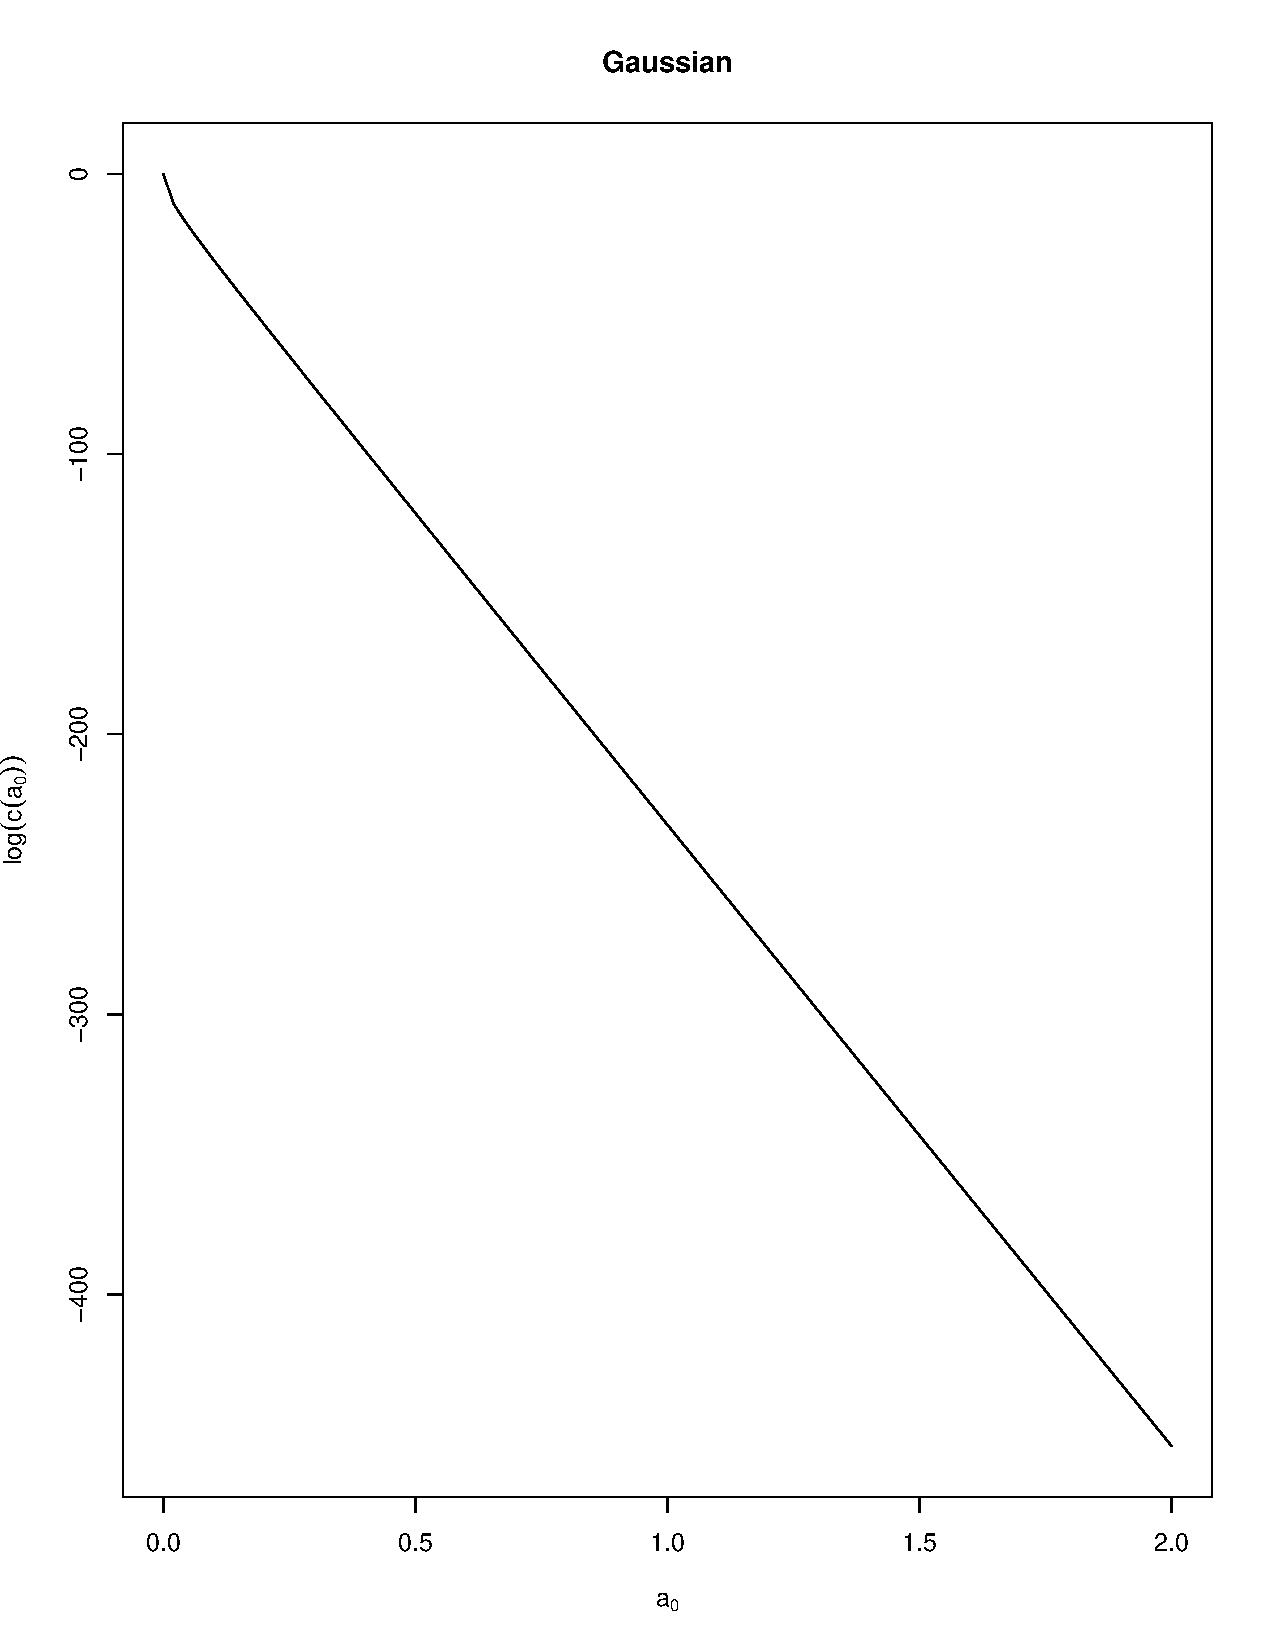
\includegraphics[width=7cm]{../figures/Gaussian.pdf}}
\hfill
\subfigure[Poisson]{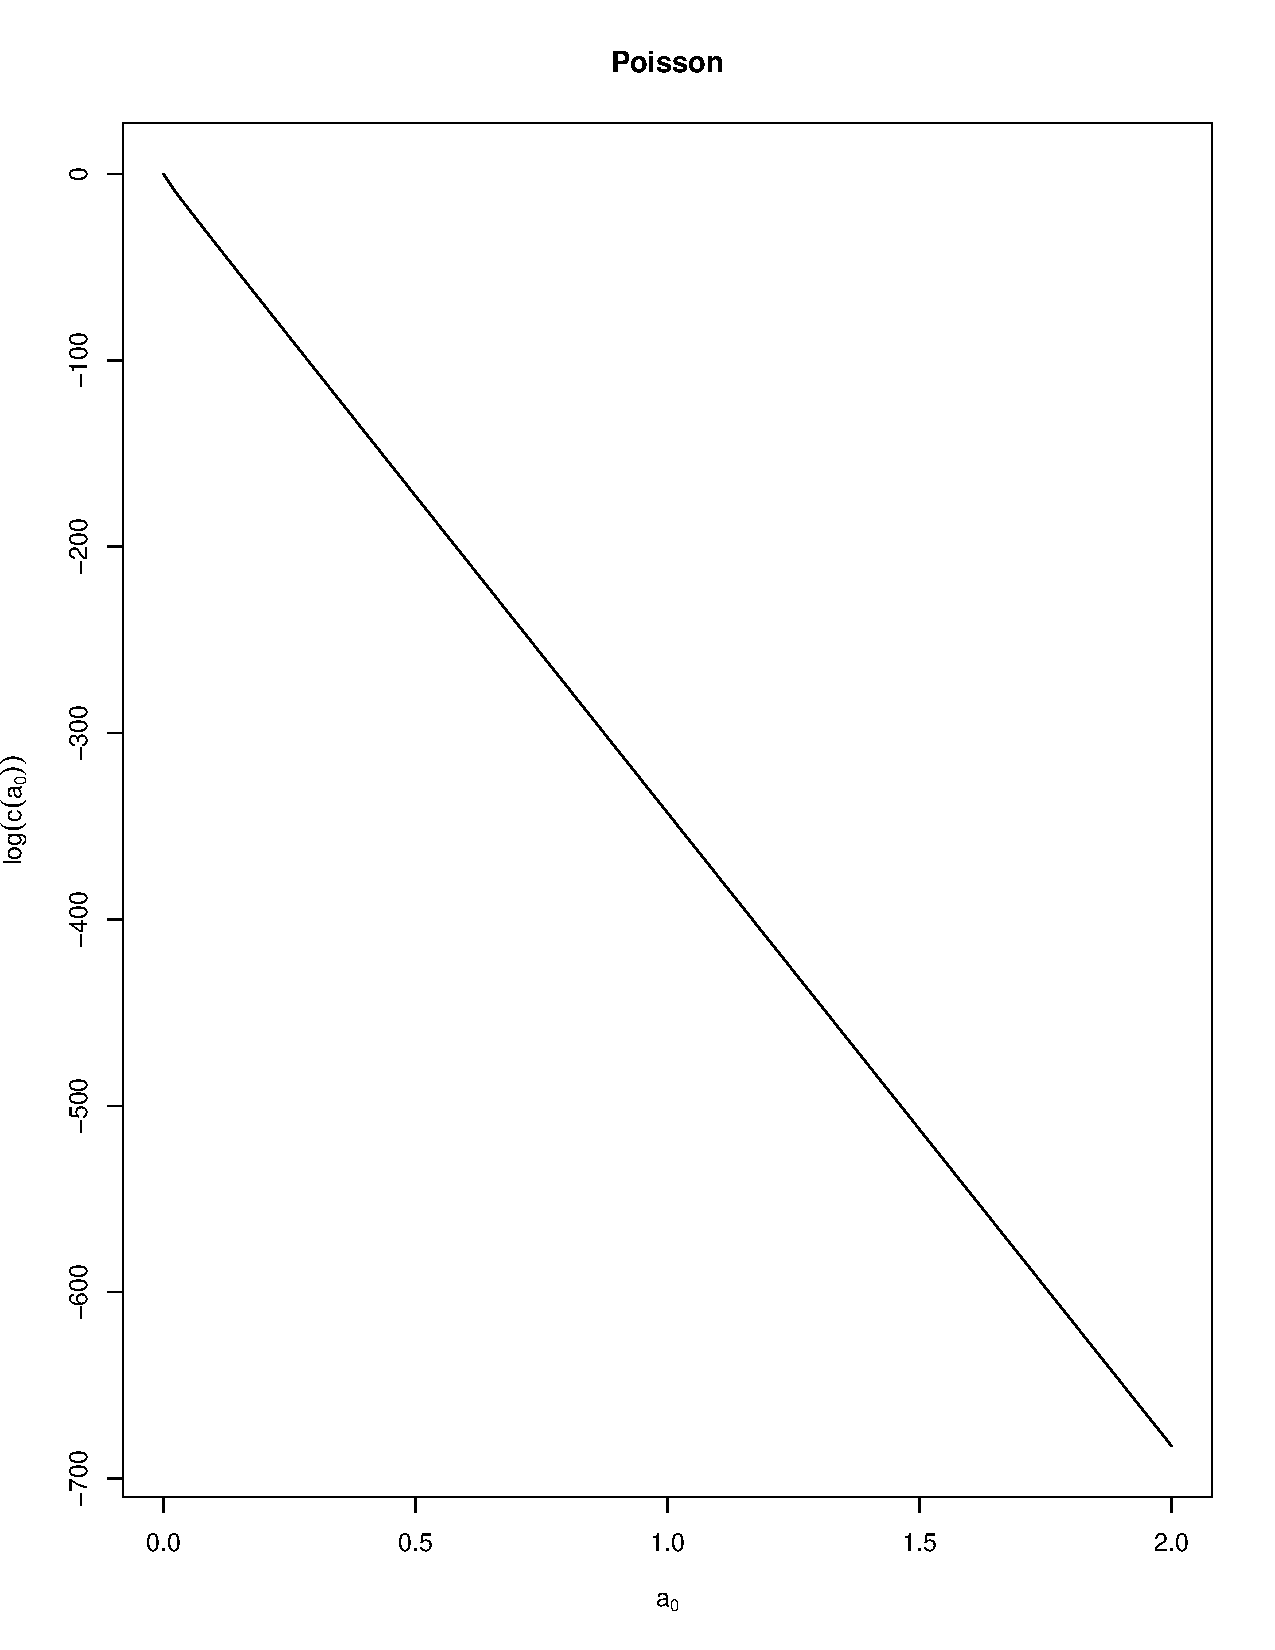
\includegraphics[width=7cm]{../figures/Poisson.pdf}}\\
\hfill
\subfigure[Bernoulli]{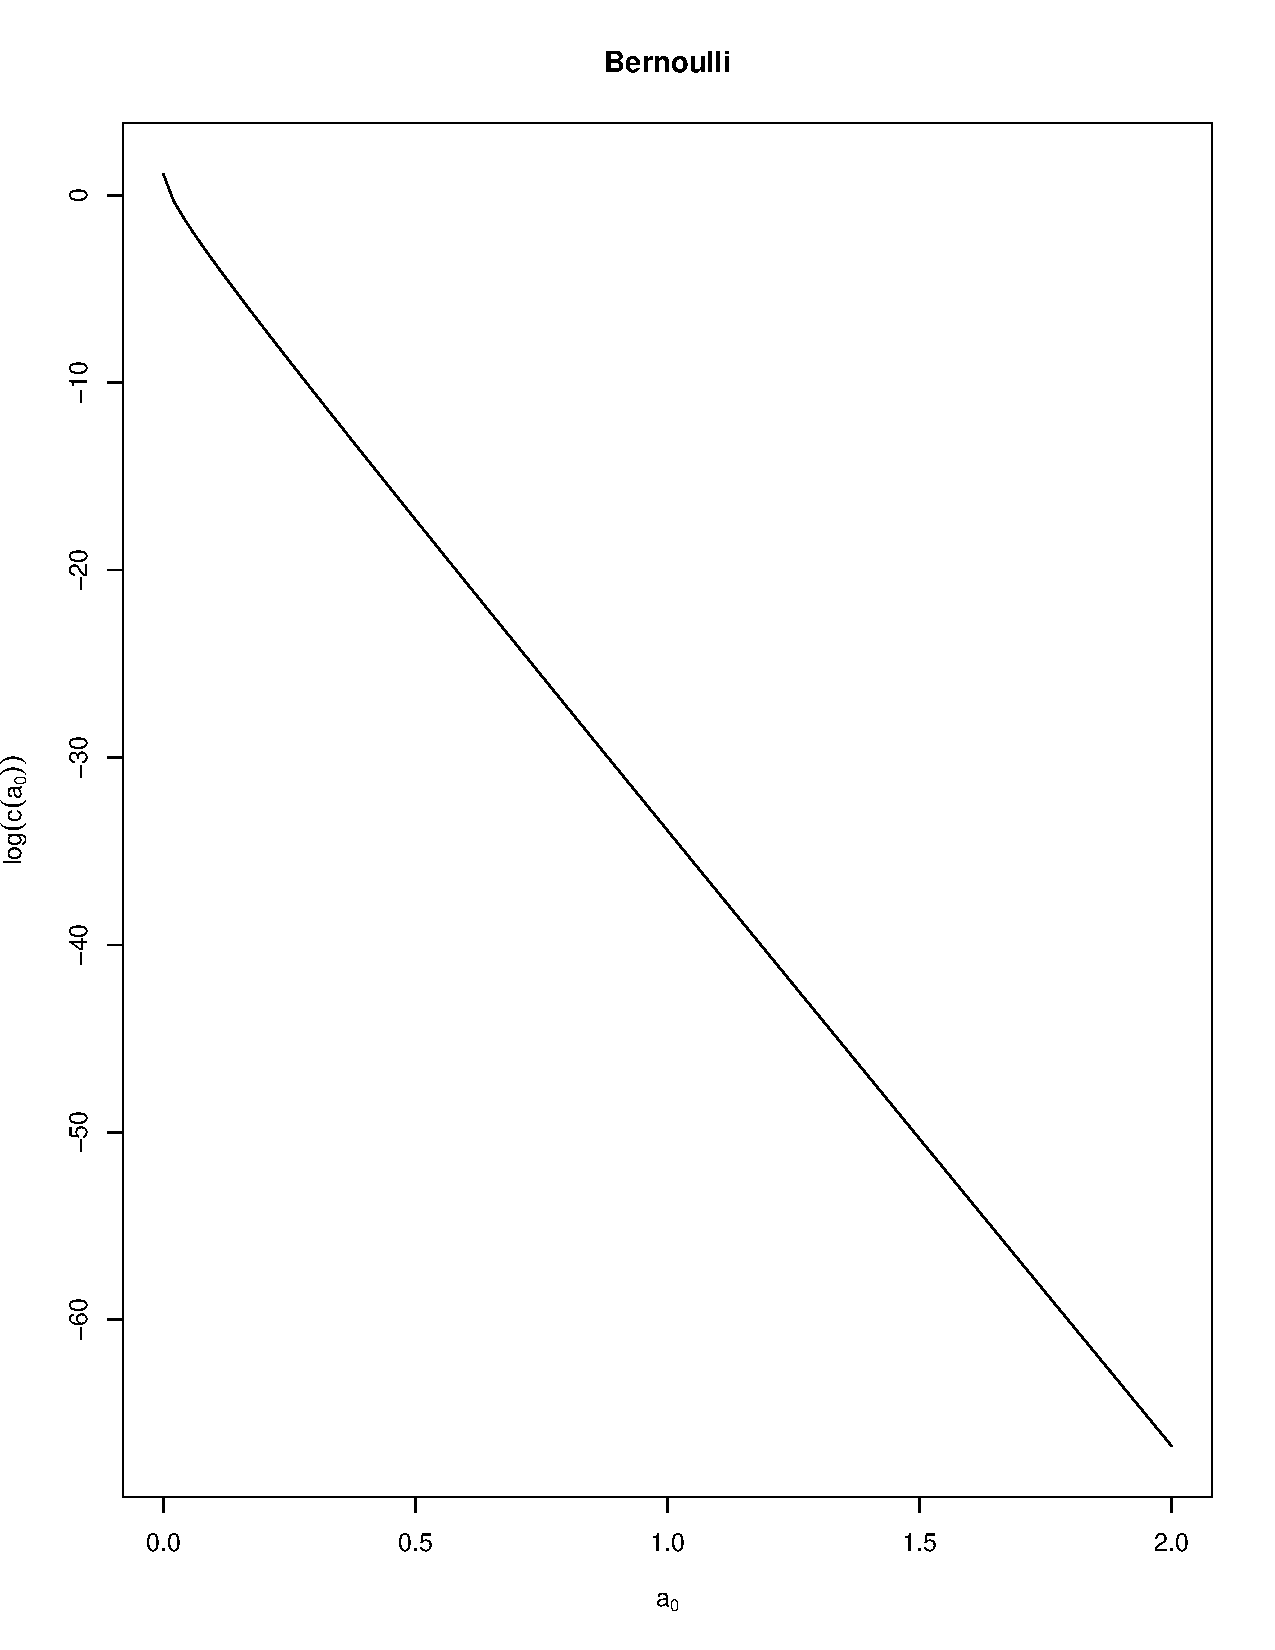
\includegraphics[width=7cm]{../figures/Bernoulli.pdf}}
\hfill
\subfigure[Inverse-Gaussian]{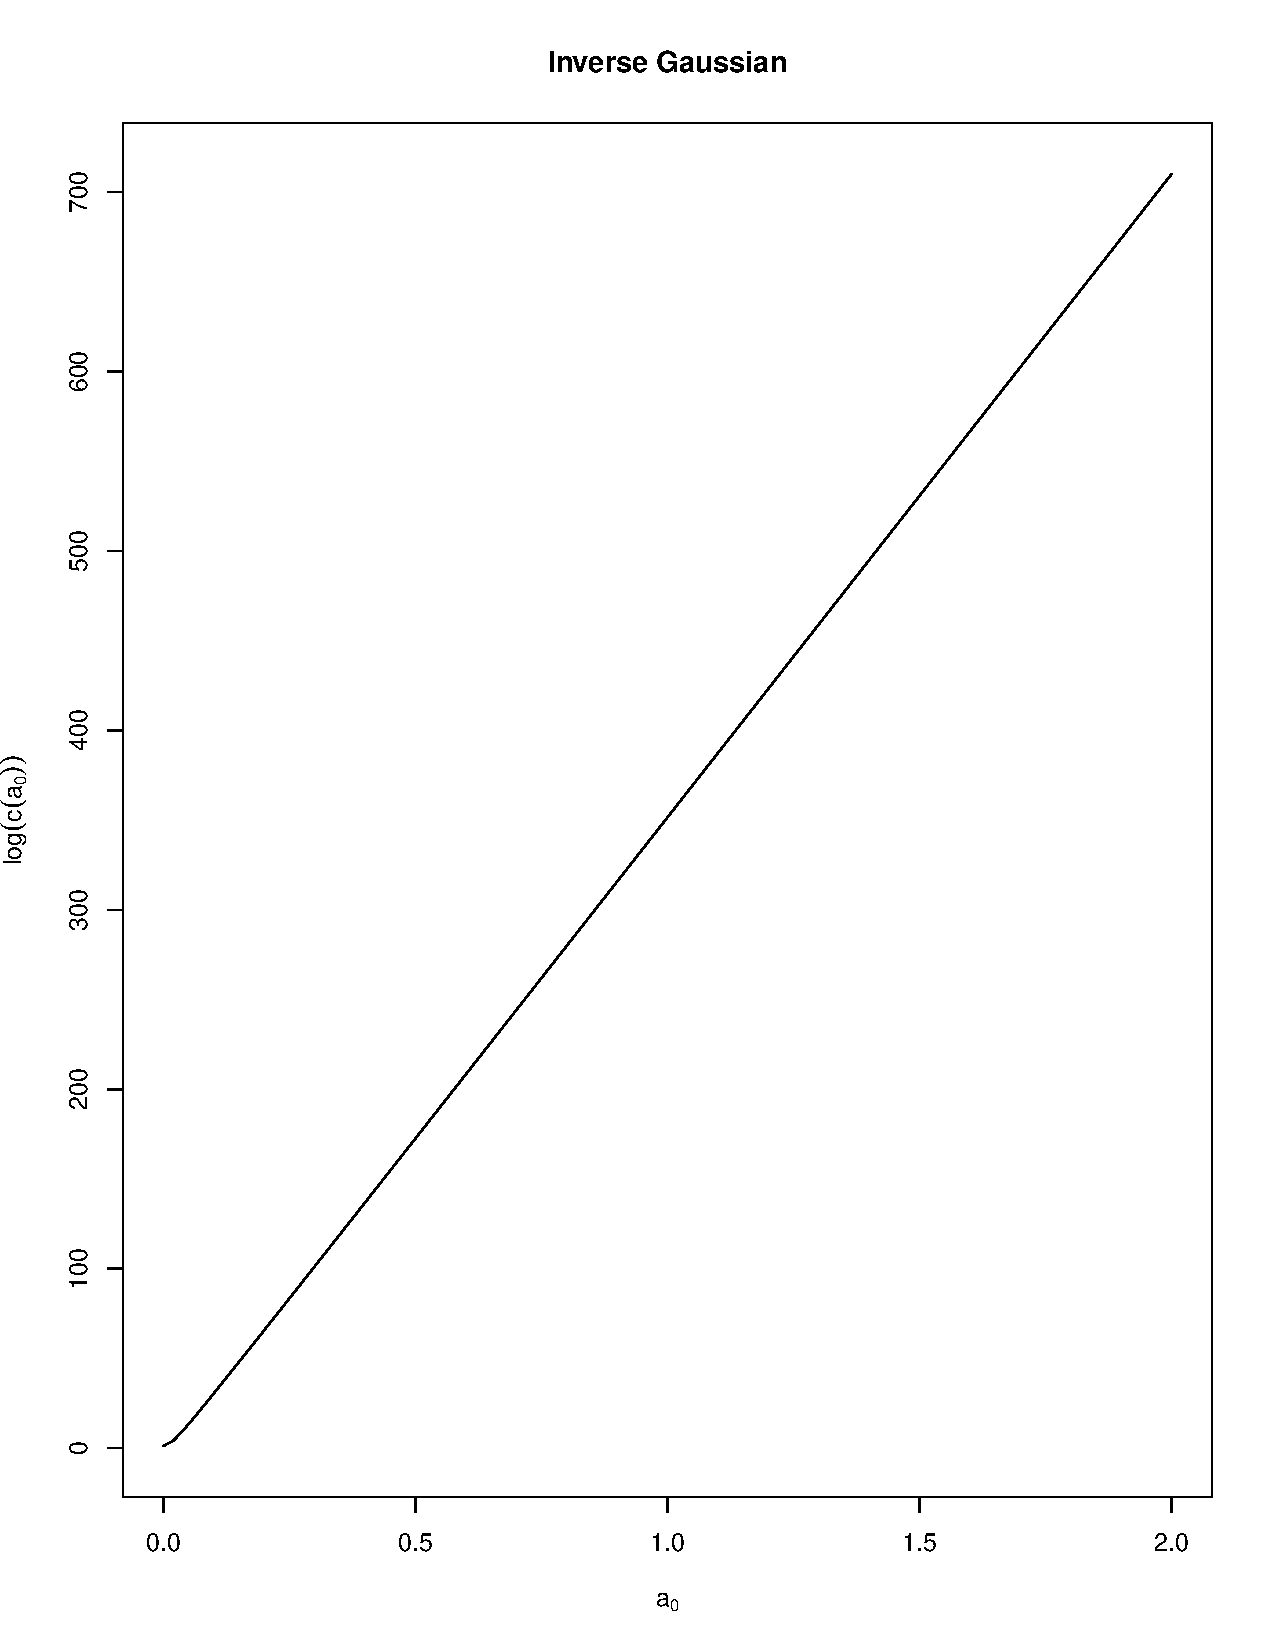
\includegraphics[width=7cm]{../figures/InverseGaussian.pdf}}
\caption{\textbf{The normalising constant $c(a_0)$ for several models}.
The plots show $\log c(a_0)$ for a host of models.
Notice how for the inverse-Gaussian model  $\log c(a_0)$ (and $c(a_0)$) is~\textbf{increasing}.
}
\label{fig:cA0}
\end{figure}

\begin{figure}
\hfill
\subfigure[Regression]{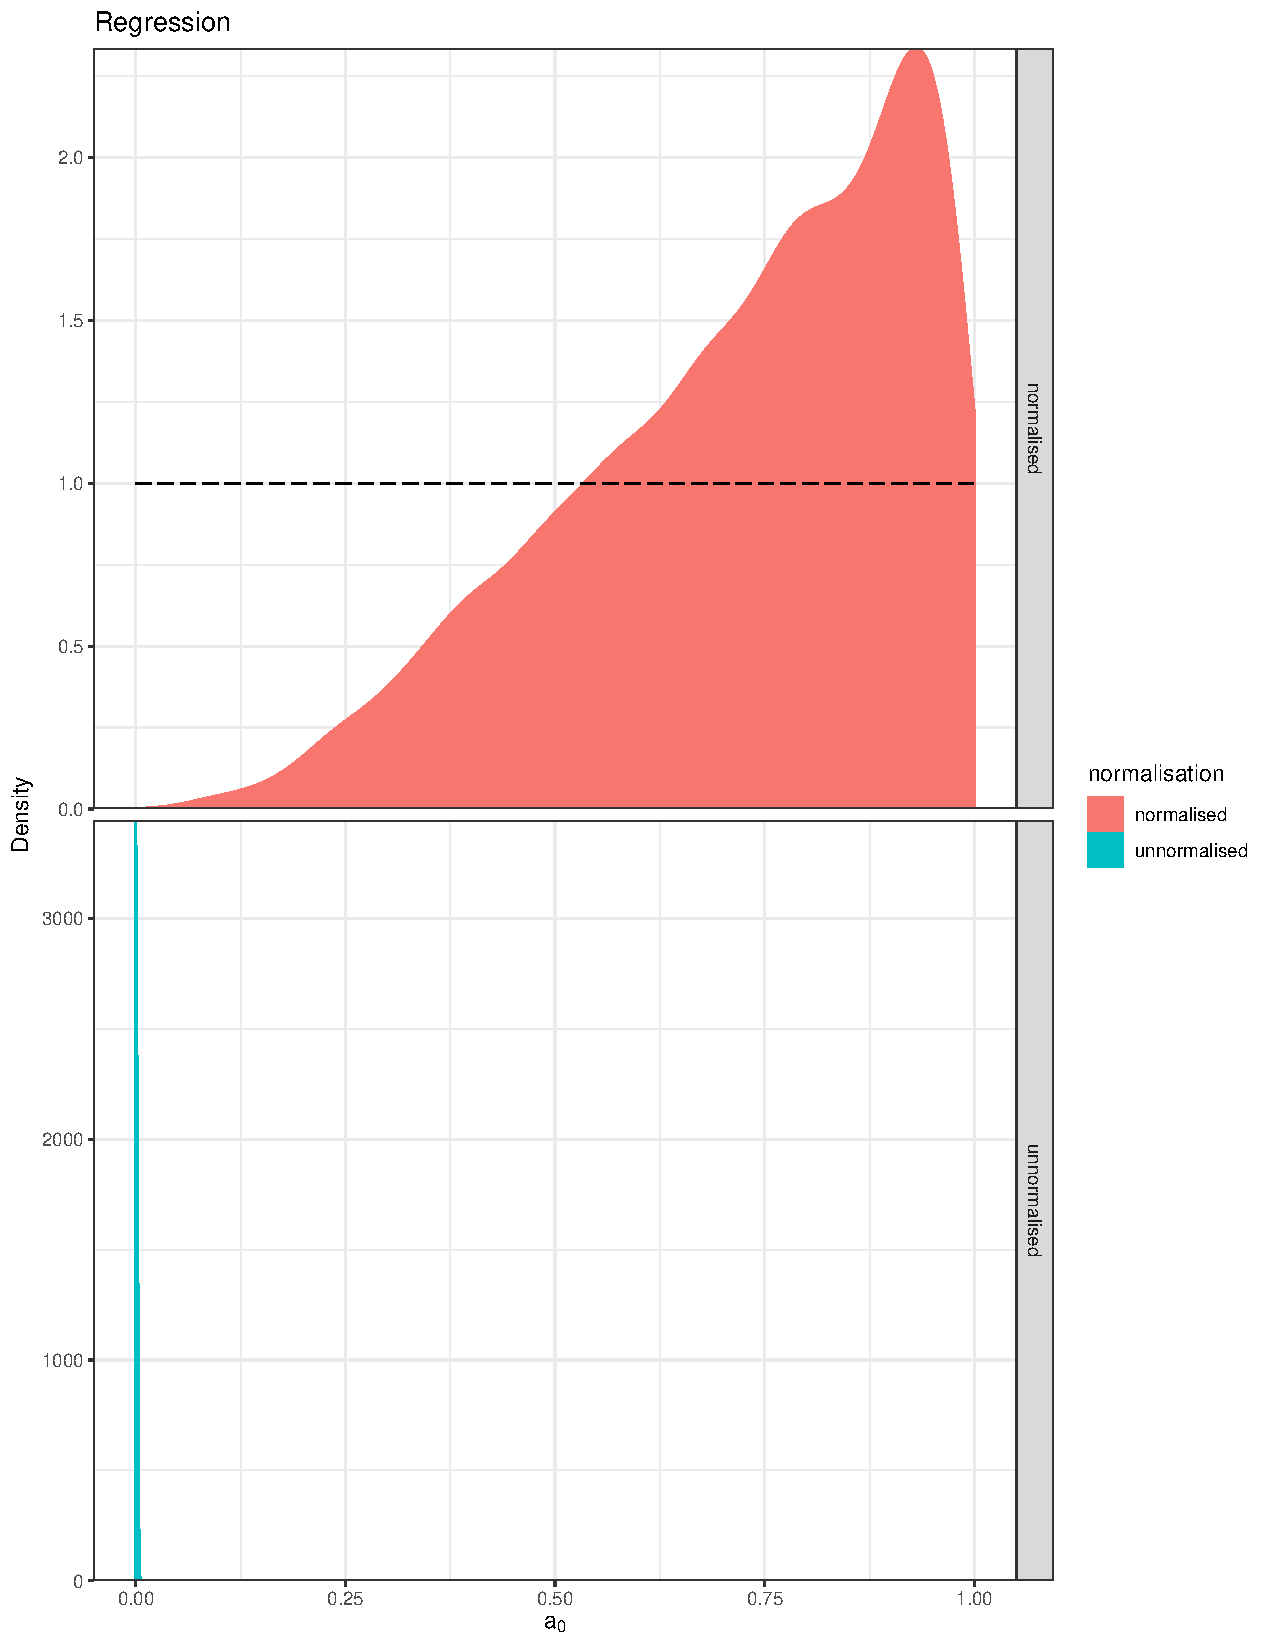
\includegraphics[width=7cm]{../figures/a0_posterior_Regression.pdf}}
\hfill
\subfigure[Poisson]{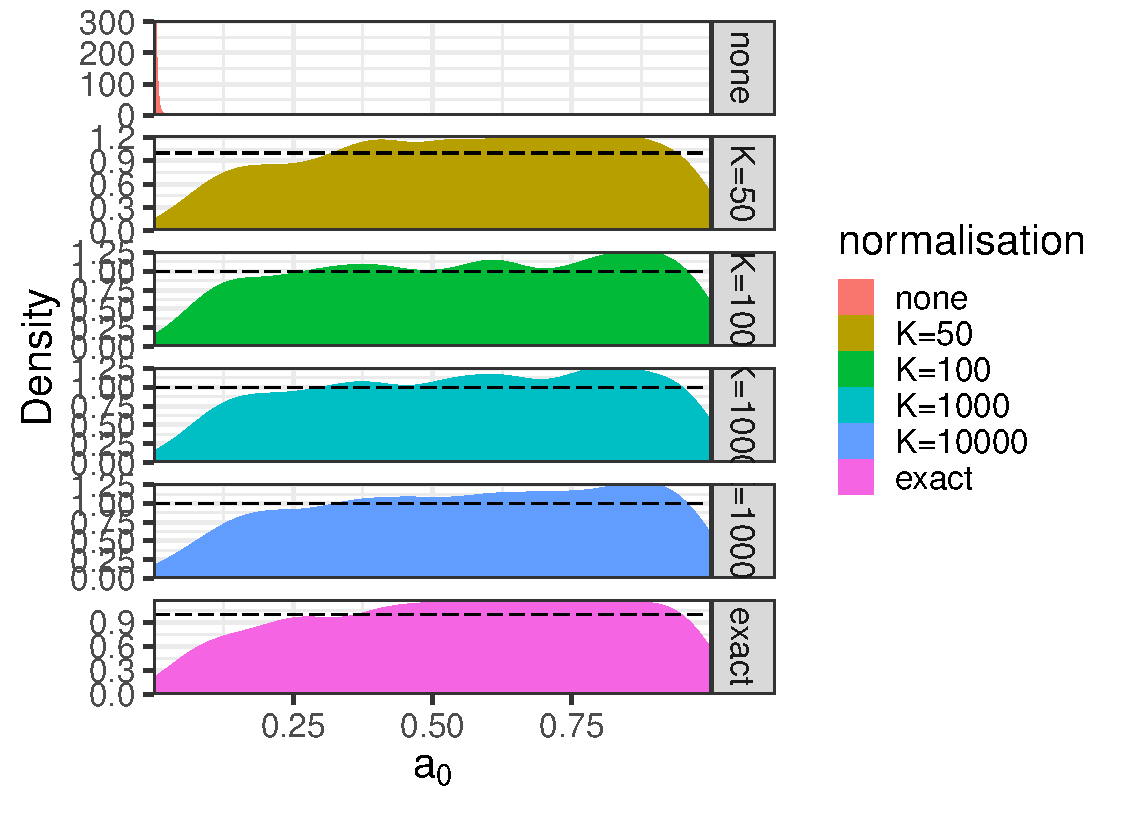
\includegraphics[width=7cm]{../figures/a0_posterior_Poisson.pdf}}\\
\hfill
\subfigure[Bernoulli]{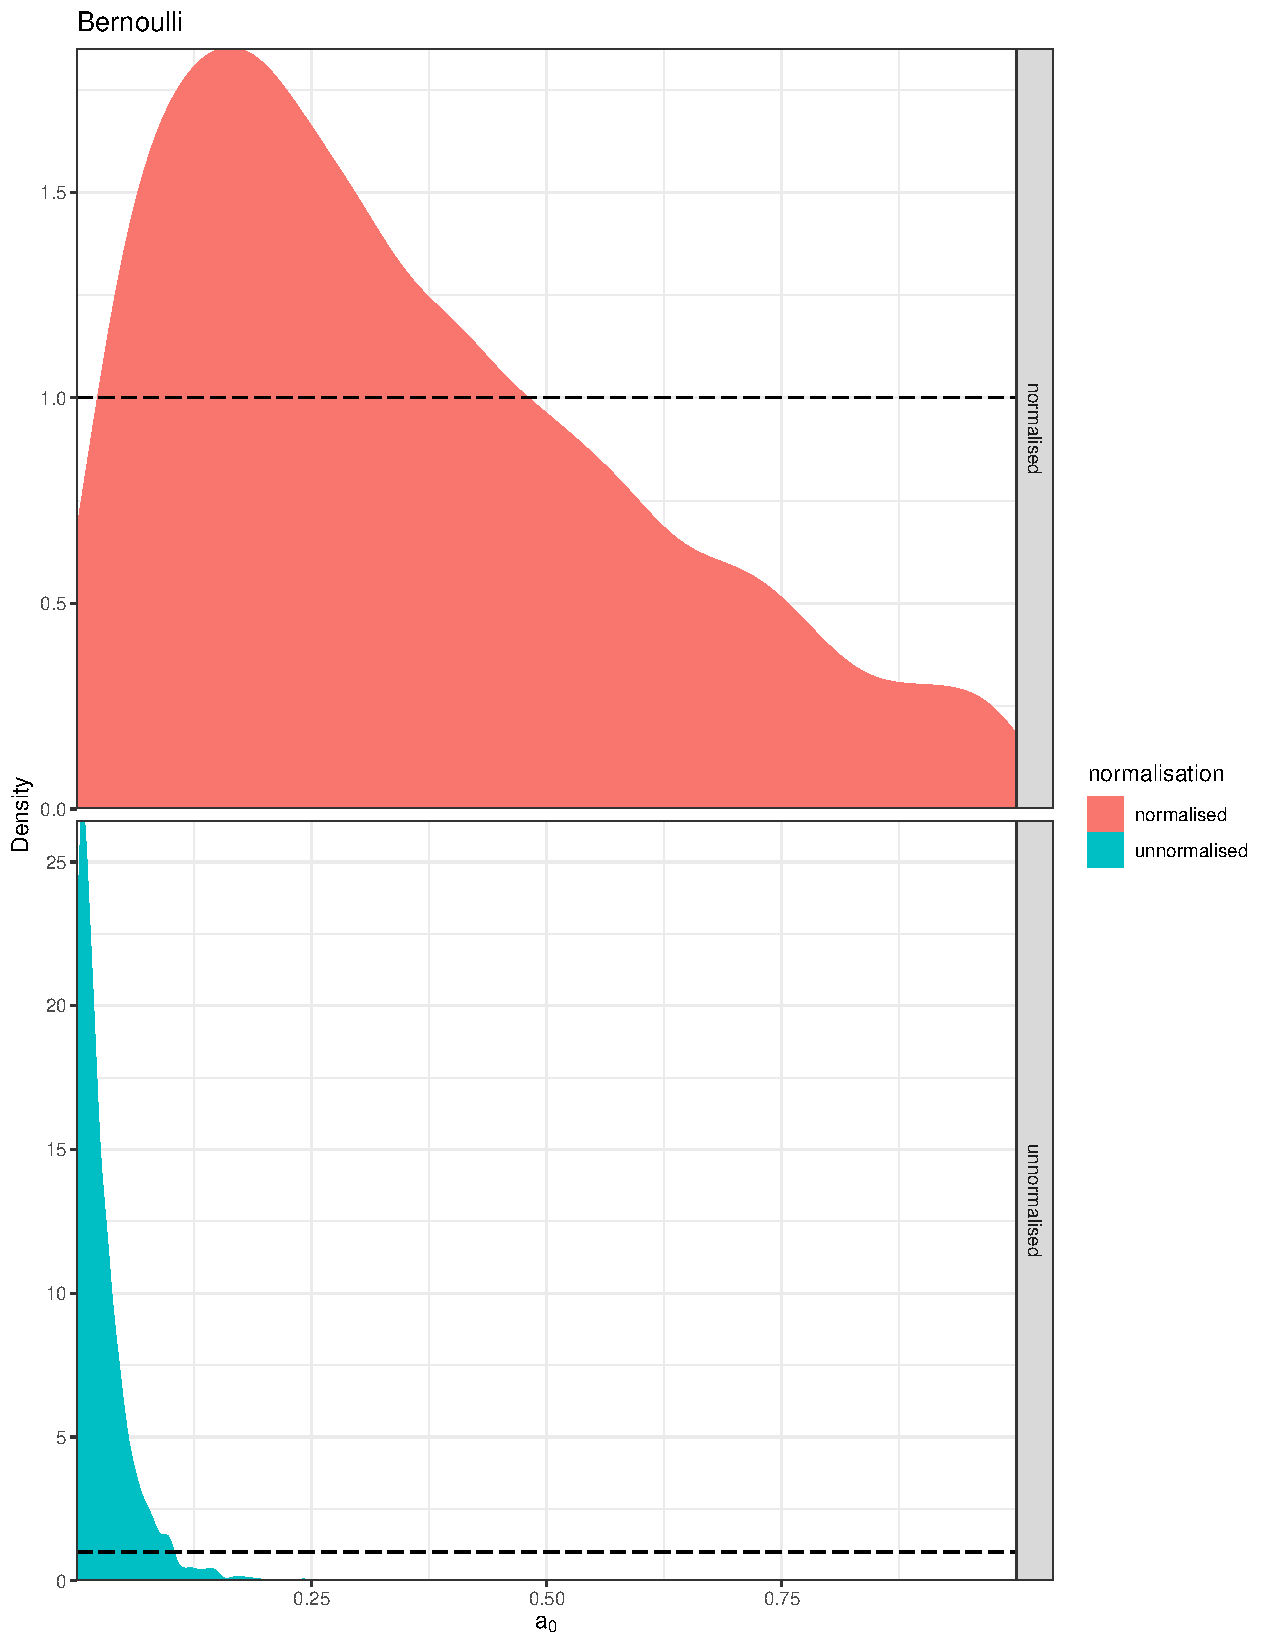
\includegraphics[width=7cm]{../figures/a0_posterior_Bernoulli.pdf}}
\hfill
\subfigure[Beta-binomial]{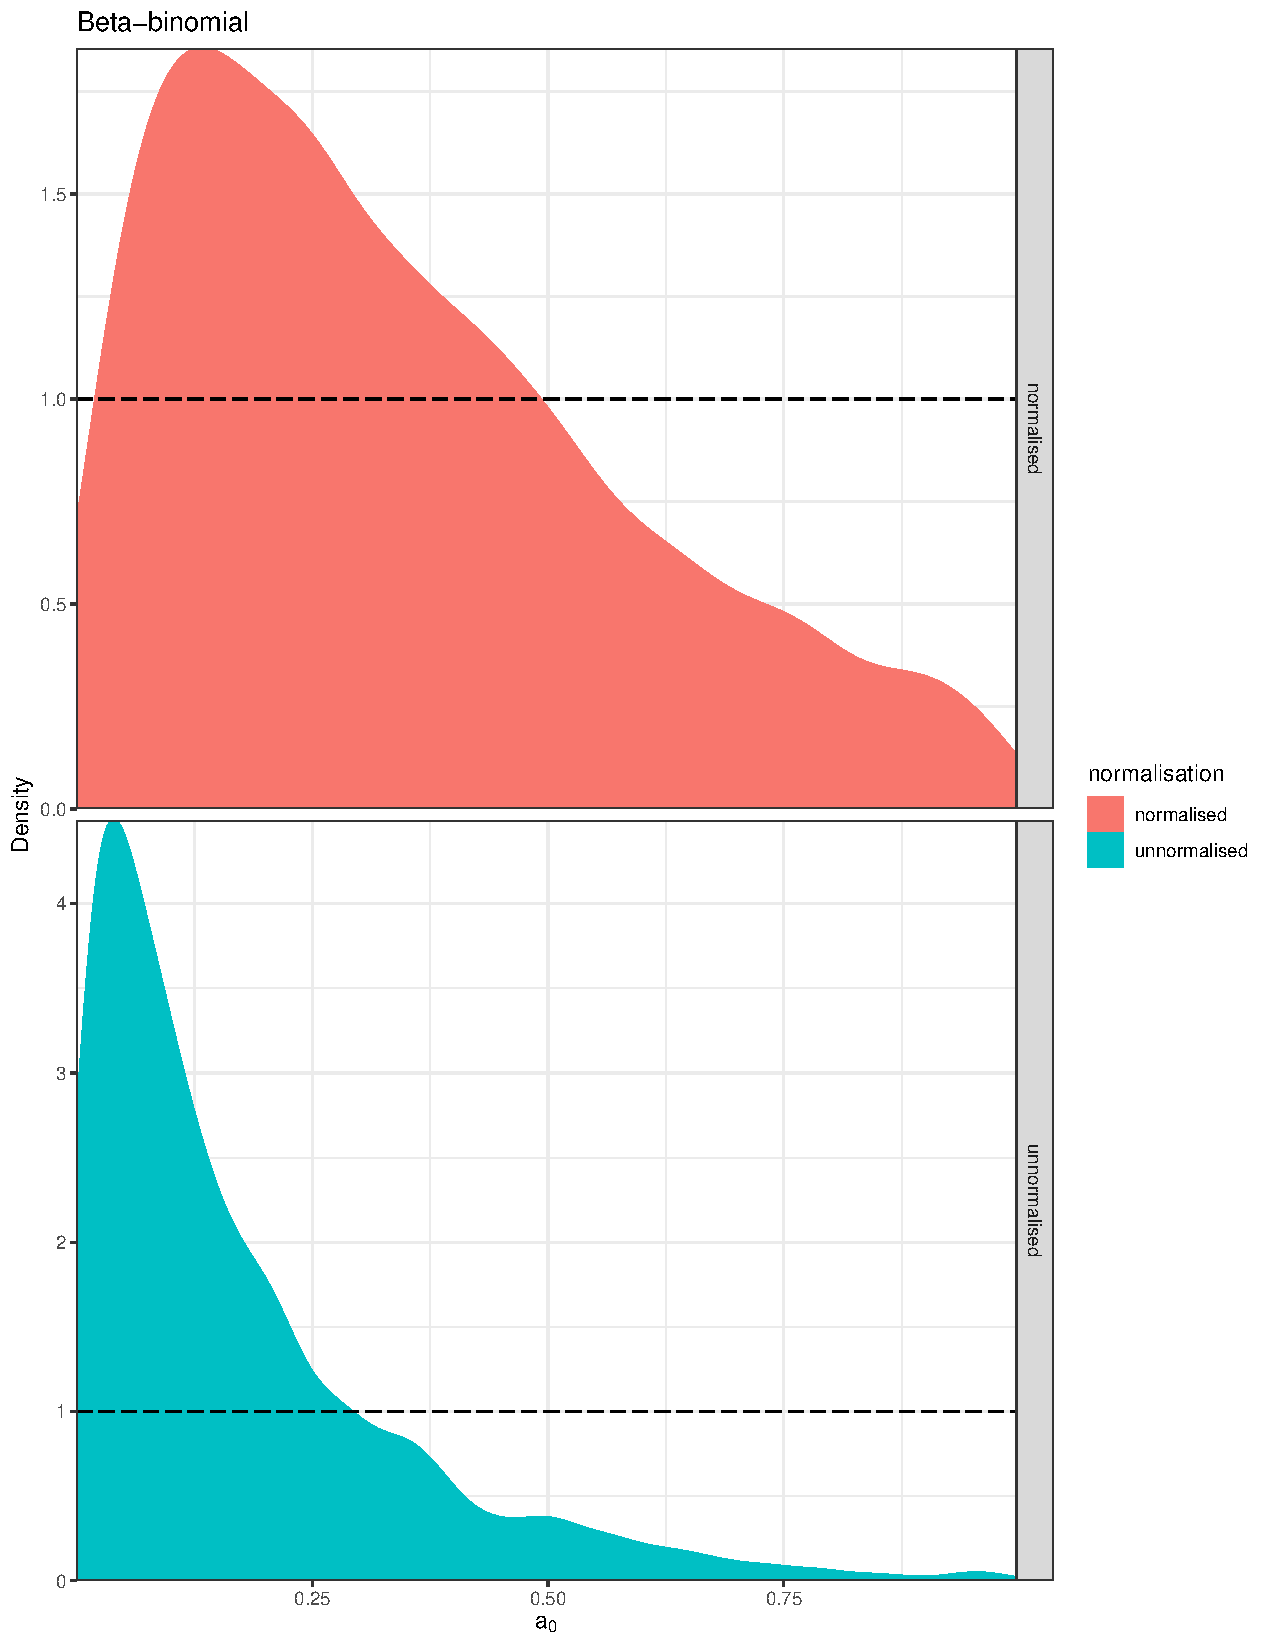
\includegraphics[width=7cm]{../figures/a0_posterior_BetaBinomial.pdf}}
\hfill
\caption{\textbf{The posterior distribution of $a_0$ under normalised and unnormalised models}.
The panels (and colours) correspond to the posterior distribution of the parameter $a_0$ when $c(a_0)$ is accounted for and when it is not included.
The Beta-binomial model is introduced here so that the reader can compare the results to those for a Bernoulli likelihood.
}
\label{fig:normalisation}
\end{figure}
\end{document}          
